\documentclass[12pt]{report}
\usepackage[T1]{fontenc}
\usepackage[utf8]{inputenc}
\usepackage{lmodern, textcomp} %textcomp for usage of euro currency symbol
\usepackage{listings}
\usepackage[margin=1in]{geometry}
\usepackage{csquotes}
\usepackage[english]{babel}
\usepackage{color}
\usepackage{xcolor} %for more colours to use in hyperref
\usepackage{amsmath}
\usepackage{makecell} %for resizing hline
\usepackage{float}
\usepackage{graphicx} %for pictures
\usepackage[caption = false]{subfig}

\graphicspath{ {figures/} }
\usepackage[
    backend=biber,
    style=numeric,
    sorting=none
    ]{biblatex}
\addbibresource{ref.bib}

\usepackage{hyperref}
\hypersetup{
    colorlinks=true, %set true if you want colored links
    linkcolor={red!50!black},
    citecolor={blue!50!black},
    urlcolor={blue!80!black}
    }
    
\usepackage{listings}
\usepackage{color}


\usepackage{graphicx}
\usepackage{caption}
\usepackage{subcaption}

\definecolor{mygreen}{rgb}{0,0.6,0}
\definecolor{mygray}{rgb}{0.5,0.5,0.5}
\definecolor{mymauve}{rgb}{0.58,0,0.82}

\lstset{ %
  backgroundcolor=\color{white},   % choose the background color; you must add \usepackage{color} or \usepackage{xcolor}; should come as last argument
  basicstyle=\footnotesize,        % the size of the fonts that are used for the code
  breakatwhitespace=false,         % sets if automatic breaks should only happen at whitespace
  breaklines=true,                 % sets automatic line breaking
  captionpos=b,                    % sets the caption-position to bottom
  commentstyle=\color{mygreen},    % comment style
  deletekeywords={...},            % if you want to delete keywords from the given language
  escapeinside={\%*}{*)},          % if you want to add LaTeX within your code
  extendedchars=true,              % lets you use non-ASCII characters; for 8-bits encodings only, does not work with UTF-8
  frame=single,	                   % adds a frame around the code
  keepspaces=true,                 % keeps spaces in text, useful for keeping indentation of code (possibly needs columns=flexible)
  keywordstyle=\color{blue},       % keyword style
  language=Octave,                 % the language of the code
  morekeywords={*,...},           % if you want to add more keywords to the set
  numbers=left,                    % where to put the line-numbers; possible values are (none, left, right)
  numbersep=5pt,                   % how far the line-numbers are from the code
  numberstyle=\tiny\color{mygray}, % the style that is used for the line-numbers
  rulecolor=\color{black},         % if not set, the frame-color may be changed on line-breaks within not-black text (e.g. comments (green here))
  showspaces=false,                % show spaces everywhere adding particular underscores; it overrides 'showstringspaces'
  showstringspaces=false,          % underline spaces within strings only
  showtabs=false,                  % show tabs within strings adding particular underscores
  stepnumber=2,                    % the step between two line-numbers. If it's 1, each line will be numbered
  stringstyle=\color{mymauve},     % string literal style
  tabsize=2,	                   % sets default tabsize to 2 spaces
  title=\lstname                   % show the filename of files included with \lstinputlisting; also try caption instead of title
}

\usepackage{algorithm}
\usepackage[noend]{algpseudocode}
\makeatletter
\def\BState{\State\hskip-\ALG@thistlm}
\makeatother

\newcommand*\samethanks[1][\value{footnote}]{\footnotemark[#1]}

\title{\Large{\textbf{Assignment 2 Report}}\\\Large{IEORE 4742 Deep Learning for OR and FE}}

\author{
    Ahmad Shayaan\thanks{All authors contributed equally to this work.} \\as5948
    } 

\date{
\{\href{mailto:ahmad.shayaan@columbia.edu}{\texttt{\small{ahmad.shayaan@columbia.edu}}}\}\texttt{\small{@columbia.edu}}\\
    Columbia University\\
    \today}



\usepackage[utf8]{inputenc}

% Default fixed font does not support bold face
\DeclareFixedFont{\ttb}{T1}{txtt}{bx}{n}{12} % for bold
\DeclareFixedFont{\ttm}{T1}{txtt}{m}{n}{12}  % for normal

% Custom colors
\usepackage{color}
\definecolor{deepblue}{rgb}{0,0,0.5}
\definecolor{deepred}{rgb}{0.6,0,0}
\definecolor{deepgreen}{rgb}{0,0.5,0}

\usepackage{listings}

% Python style for highlighting
\newcommand\pythonstyle{\lstset{
		language=Python,
		basicstyle=\ttm,
		otherkeywords={self},             % Add keywords here
		keywordstyle=\ttb\color{deepblue},
		emph={MyClass,__init__},          % Custom highlighting
		emphstyle=\ttb\color{deepred},    % Custom highlighting style
		stringstyle=\color{deepgreen},
		frame=tb,                         % Any extra options here
		showstringspaces=false            % 
	}}
	
	
	% Python environment
	\lstnewenvironment{python}[1][]
	{
		\pythonstyle
		\lstset{#1}
	}
	{}
	
	% Python for external files
	\newcommand\pythonexternal[2][]{{
			\pythonstyle
			\lstinputlisting[#1]{#2}}}
	
	% Python for inline
	\newcommand\pythoninline[1]{{\pythonstyle\lstinline!#1!}}

\begin{document}

\maketitle
%\tableofcontents

\pagebreak

\chapter*{Question 1 Solution }

\section*{Question 1 Part 1}

The total number of trainable parameters is the sum of all the wights and biases of each layer. In the network that we are training the total number of parameters are given by.

\begin{equation*}
	\resizebox{.9\hsize}{!}{
		\text{Total Number of Parameters} = $(784 \times 400) + 400 + (400 \times 200) + 200 + (200 \times 100) + 100 + (100 \times 50) + 50 + (50 \times 25) + 25 + (25 \times 10) + 10$  
	}
\end{equation*}

\begin{equation*}
\text{Total Number of Parameters} = 420885
\end{equation*}
	
\section*{Question 1 Part 2}
\begin{table}[H]
	\centering
	\caption{Change in accuracy with change in architecture}
	\resizebox{.9\textwidth}{!}{
	\begin{tabular}{|c|c|c|c|c|}
		\hline
		Layers         & Architecture 1     & Architecture 2     & Custom Architecture 1 & Custom Architecture 2 \\ \hline
		Hidden Layer 1 & Sigmoid (784x400)  & Tanh (784x400)     &   ReLu (784x500 )   &  ReLu (784x1000)  \\ \hline
		Hidden Layer 2 & Tanh (400x200)     & ReLu (400x200)     &   ReLu  (500x400)   &  ReLu (1000x500)      \\ \hline
		Hidden Layer 3 & ReLu (200x100)     & ReLu (200x100)     &   ReLu  (400x200)   &  ReLu (500x400)      \\ \hline
		Hidden Layer 4 & Sigmoid (100x50)   & Tanh (100x50)      &   ReLu  (200x100)   &  ReLu (400x200)     \\ \hline
		Hidden Layer 5 & Leaky ReLu (50x25) & Leaky ReLu (50x25) &   ReLu  (100x50)    &  ReLu (200x100)    \\ \hline
		Hidden Layer 6 & None               & None               &   ReLu  (50x25)     &  ReLu (100x50)       \\ \hline
		Hidden Layer 7 & None               & None               &        None         &  ReLu (50x25)   \\ \hline
		Accuracy       & 97.93              & 98.16              &         98.4       &   98.62           \\ \hline
	\end{tabular}
	}

	\label{tb:1}
\end{table}

It can be observed from the table that having ReLU activation and more number of layers increases the accuracy. This is because ReLU activation does not saturate the gradient which help the optimizer to quickly converge to the optimum. Increase in the depth of the network helps the network learn more complex relationship between the input features and the objective function. 

\section*{Question 1 Part 3}\label{part13}

\begin{table}[H]
	\centering
	\caption{Accuracy for different optimizers}
	\begin{tabular}{|l|l|}
		\hline
		Optimizer Used             & Accuracy in percentage \\ \hline
		Gradient Descent Optimizer & 98.12                  \\ \hline
		Adam Optimizer             & 10.09                  \\ \hline
		Adagrad Optmizer           & 98.27                  \\ \hline
		RMSprop Optimizer          & 10.1                   \\ \hline
	\end{tabular}
	\label{tb:2}
\end{table}

It can be seen from the table that Adagrad optimizer does the best with the same network architecture. This is because this algorithm adaptively scales the learning rate for each step it takes towards the optimum. Adam and RMSprop algorithm don't do as well because the learning rate is not sufficient. On reducing the learning rate I observed that Adam and RMS prop do better than other optimization algorithms. It has been shown that Adam and RMSProp are highly sensitive to certain values of the learning rate and they can catastrophically fail to converge. Gradient Descent optimizer has also provided us with good results.


\chapter*{Question 2}

\section*{Question 2 Part 2}
The linearly interpolated loss surfaces of the different networks are shown below. To plot the surface I modified the linear interpolation code that was provided to us. 


\begin{figure}[H]
	\subfloat[Gradient optimzer]{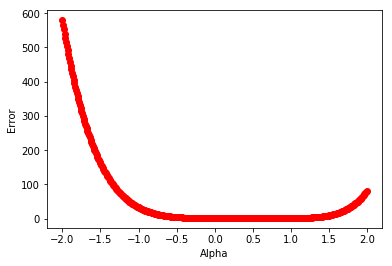
\includegraphics[width = 3in]{1}} 
	\subfloat[Adam optimizer]{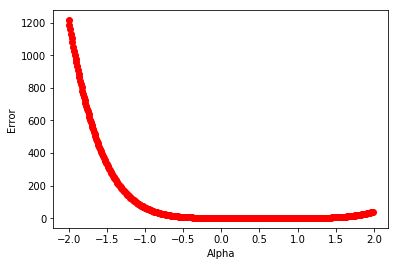
\includegraphics[width = 3in]{2}}\\
	\subfloat[Adagrad Optimizer]{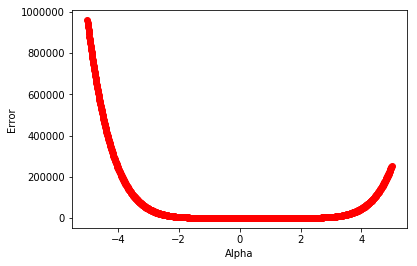
\includegraphics[width = 3in]{3}}
	\subfloat[RMSProp Optimizer]{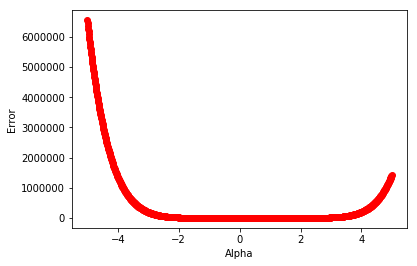
\includegraphics[width = 3in]{4}} 
	\caption{Loss Function for various optimizers}
	\label{fig:1}
\end{figure}

Figure~\ref{fig:1}a shows the loss surface for the first network in question 1. It can be observed from the figure that the loss surface is flat near the optimum learned by our network and tends to rise as we move further away from the center.  


Figure~\ref{fig:1}b shows the loss surface for the second network in question 1. The curve again is flat at the optimum learned by the network and rises as we move away from the center. However, the rate at which the cost rise smaller as compared to the loss surface with previous parameters. 



Figure~\ref{fig:1}c shows the loss surface for the network with six layers in question 1. There is no change in the loss surface as we wary the interpolation factor from -2 to 2. We can only observe the changes in the loss surface if we increase the range of the interpolation factor. On increasing the rage we can observe that the loss rapidly start rising as we move away from the optimum. 

Figure~\ref{fig:1}d shows the loss surface for the network with seven layers. It can be observed that the rate of change of the loss as we vary the interpolation parameter is smaller compared to the loss surface for the six layer network.	 

\section*{Question 2 Part 2}
In this question we had to plot the change in the loss surface as we change the optimization algorithm.


\begin{figure}[H]
	\subfloat[Gradient optimzer]{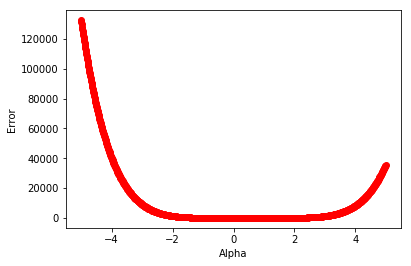
\includegraphics[width = 3in]{gradient}} 
	\subfloat[Adam optimizer]{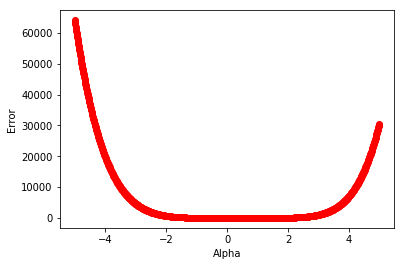
\includegraphics[width = 3in]{adam}}\\
	\subfloat[Adagrad Optimizer]{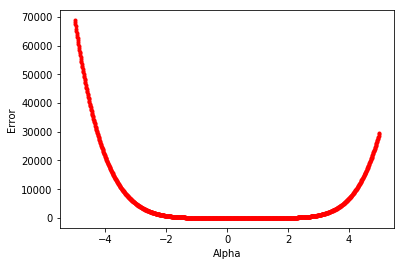
\includegraphics[width = 3in]{adagrad}}
	\subfloat[RMSProp Optimizer]{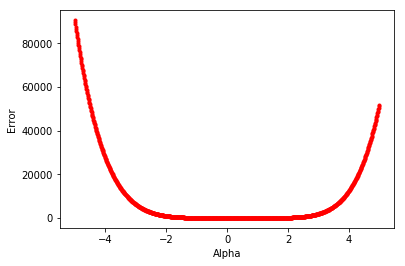
\includegraphics[width = 3in]{RMSprop}} 
	\caption{Loss Function for various optimizers}
	\label{fig:2}
\end{figure}

Figure~\ref{fig:2} shows the loss surfaces for different optimizers. The loss surfaces mostly differ on the rate with which the loss changes as we change interpolation factor. The rate of change on of the loss is maximum in case of gradient descent optimizer and minimum in case Adagrad optimizer


\chapter*{Question 3}

\section*{Question 3 Part 1}
The total number of trainable parameters is the sum of all the wights and biases of each layer. In the network that we are training the total number of parameters are given by.

\begin{equation*}
\resizebox{.9\hsize}{!}{
	\text{Total Number of Parameters} = $(3072 \times 400) + 400 + (400 \times 200) + 200 + (200 \times 100) + 100 + (100 \times 50) + 50 + (50 \times 25) + 25 + (25 \times 10) + 10$  
}
\end{equation*}

\begin{equation*}
\text{Total Number of Parameters} = 1336085
\end{equation*}


\section*{Question 3 Part 2}
We had to train a network to correctly classify the images in CIFAR-10 data set. The dataset consist of 60000 images each with dimension $32\times32\times3$. The images presented in the dataset belong to 10 different classes and all the classes are mutually exclusive. There are 50000 training images and 10000 test images.
\begin{figure}[H]
	\centering
	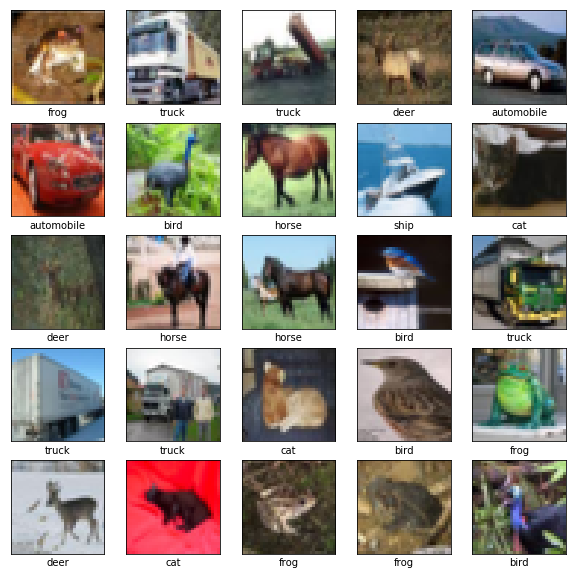
\includegraphics[width=0.5\textwidth]{CIFAR}
	\caption{Images present in CIFAR-10 dataset}
\end{figure}

\begin{table}[H]
	\centering
	\caption{Change in accuracy with change in architecture}
	\resizebox{.9\textwidth}{!}{
		\begin{tabular}{|c|c|c|c|c|}
			\hline
			Layers         & Architecture 1     & Architecture 2     & Custom Architecture 1 & Custom Architecture 2 \\ \hline
			Hidden Layer 1 & Sigmoid (3072x400)  & Tanh (3072x400)     &   ReLu (3072x1000)   &  ReLu (3072x1000)  \\ \hline
			Hidden Layer 2 & Tanh (400x200)     & ReLu (400x200)     &   ReLu  (1000x500)   &  ReLu (1000x500)      \\ \hline
			Hidden Layer 3 & ReLu (200x100)     & ReLu (200x100)     &   ReLu  (500x200)   &  ReLu (500x400)      \\ \hline
			Hidden Layer 4 & Sigmoid (100x50)   & Tanh (100x50)      &   ReLu  (200x100)   &  ReLu (400x200)     \\ \hline
			Hidden Layer 5 & Leaky ReLu (50x25) & Leaky ReLu (50x25) &   ReLu  (100x50)    &  ReLu (200x100)    \\ \hline
			Hidden Layer 6 & None               & None               &   ReLu  (50x25)     &  ReLu (100x50)       \\ \hline
			Hidden Layer 7 & None               & None               &        None         &  ReLu (50x25)   \\ \hline
			Accuracy       & 26.94              &  27.4               &         40       &    47.63        \\ \hline
		\end{tabular}
	}
	
	\label{tb:3}
\end{table}

It can be observed from table~\ref{tb:3} that accuracy increases with the increase in the depth of the network and the number of neurons. This is because a deeper network is able to capture more complex  relationship between the input features and the objective function. The accuracy also increases with the increase in the number of neurons at each layer as with more number of neurons per layer we will be loosing very less information when we reduce the dimensionality of the input. 

\section*{Question 3 Part 3}

\begin{table}[H]
	\centering
	\caption{Accuracy for different optimizers}
	\begin{tabular}{|l|l|}
		\hline
		Optimizer Used             & Accuracy in percentage \\ \hline
		Gradient Descent Optimizer & 22.4                   \\ \hline
		Adam Optimizer             & 16                     \\ \hline
		Adagrad Optmizer           & 26.94                  \\ \hline
		RMSprop Optimizer          & 6.12                   \\ \hline
	\end{tabular}
	\label{tb:2}
\end{table}

The results replicate the findings in question one part 3 that Adagrad optimizer outperform all the other optimization function. 

\end{document}